%************************************************
\chapter{Simulation of Functional Brain Images}\label{ch:simulation}
%************************************************
In Chapter~\ref{ch:swpca}, we proposed a novel methodology for eliminating inhomogeneities due to acquisition site in multi-centre datasets. This is a good approach for \ac{MRI} images, but still requires a large recruitment procedure and individual analyses and assessments. In this chapter, we propose a simulation procedure (see Figure~\ref{fig:simulationSchema}) intended to synthesize completely new samples of an existing database that share the same properties as the original set of subjects belonging to a certain class.  

Our system is focused on nuclear imaging techniques such as \ac{PET} or \ac{SPECT}, using \ac{PCA} to project the dataset to the eigenbrain space and a statistical distribution estimator to model the distribution of the brains and classes in this new space. Once the statistical distribution of the classes is known, we can generate new coordinates on the eigenbrain space belonging to the same class, that can be then projected to the brain space.
 
\begin{figure}[htp]
	\centering
	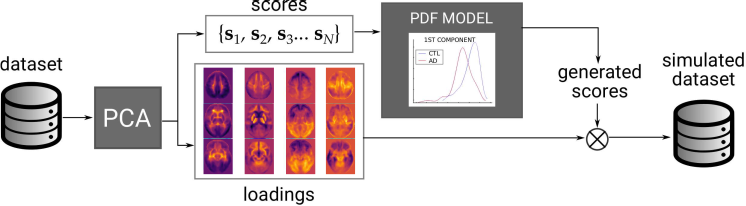
\includegraphics[width=\textwidth]{Graphics/ch8/SchemaGeneration}
	\caption{Schema of the brain image synthesis algorithm.}
	\label{fig:simulationSchema}
\end{figure} 

We have evaluated our proposed system on two modalities: FDG-\ac{PET} images from the ADNI-PET dataset and \ac{SPECT}-DaTSCAN from the PPMI-DAT database. We have tested the images under three different experiments that estimate the relation between the simulated and the real images, the ability of the simulated dataset to predict the outcome of real datasets, or the uncertainty introduced by the simulation procedure. 

For our brain synthesis algorithm to work, the source datasets must share certain characteristics: to be spatially normalized (which we did by using the SPM8 software) and intensity normalized, using normalization to the maximum strategy, which proved to be very useful in most applications \cite{Martinez-Murcia20129676,martinez2014parametrization} (see Chapter~\ref{ch:preprocessing} for more details).

\section{Simulation Methodology}
\subsection{\acs{PCA} Decomposition}
The first step of the simulation pipeline is the analysis of the dataset that we want to use as a reference. In order to do so, we project the dataset from its original image space to a lower dimensional space using \ac{PCA}, a very extended tool for analysis and feature extraction in neuroimaging \cite{Illan2011,Khedher2015}, and that was already defined at Section~\ref{sec:pca}.

In this chapter, we use the component score matrix $\mathbf{S}$, or the coordinates of the database samples in the eigenbrain space, to estimate per-class and per-component statistical distributions from which the new samples, from which we can generate new coordinates. For efficiency, and without loss of generality, we will use only the first $C$ components of the \ac{PCA} decomposition. 

\subsection{Density Estimation}
Once the images have been projected to the eigenbrain space, we want to generate new samples in this new space, in order to synthesize new images. To do so, we assume that the coordinates of the subjects of a certain class in the eigenbrain space are different realizations of a random process with a given \ac{PDF}. 

In order to estimate the \ac{PDF} of the process that generates the coordinates of each class, we use two different density estimation procedures: the model of this distribution using a Multivariate Normal Distribution, and the empirical Kernel Density Estimation. 

\subsubsection{\acf{MVN}}
The \acf{MVN}, also known as Multivariate Gaussian Distribution, is a generalization of the random normal distribution to $n$ dimensions. 

Let us note $\mathbf{S}^{c}$ the matrix containing only the coordinates in the eigenbrain space of individuals belonging to class $c$. That way, $\mathbf{S}^{i,c}$ would be the vector containing the $i^{th}$ coordinate of $\mathbf{S}^{c}$, a vector with mean $\mu^{i,c}$ and covariance matrix $\boldsymbol{\Sigma}^{i,c}$. The \ac{PDF} of that combination of coordinate and class would be: 

\begin{equation}
\hat{f}_{mvn}^{i,c}(x) = \frac{1}{(2\pi)^{N/2}\left|\boldsymbol{\Sigma}^{i,c}\right|^{1/2}} \exp{ \left(\frac{(x-\mu^{i,c})^T \boldsymbol{\Sigma}_{i,c}^{-1}(x-\mu^{i,c})}{2}\right)}
\end{equation}

\subsubsection{\acf{KDE}}
\acf{KDE} is an increasingly used method to estimate the \ac{PDF} of a set of data \cite{Botev2010,Simonoff2012}. The \ac{KDE} estimates the probability density function of the $i^{th}$ coordinate of class $c$ as: 
\begin{equation}
\hat{f}_{kde}^{i,c}(x) = \frac{1}{N_c}\sum_{l=1}^{N_c} K_h \left(x - \mathbf{S}^{i,c}_l\right) = \frac{1}{N_c h} \sum_{l=1}^{N_c} K\left(\frac{x-\mathbf{S}^{i,c}_l}{h}\right),
\end{equation}
where $l=1,\dots N_c$, with $N_c$ the number of subjects belonging to class $c$, and $\mathbf{S}^{i,c}$ contains the $i^{th}$ coordinate of $\mathbf{S}^{c}$, as in the latter section. The kernel $K(x)$ is a function of $\mathbb{R}^n$ that must define a probability: 
\begin{equation}
\idotsint_{\mathbb{R}^n} K(\mathbf{x}) d\mathbf{x} = 1
\end{equation}
It also must be centred:
\begin{equation}
\idotsint_{\mathbb{R}^n} \mathbf{x}K(\mathbf{x}) d\mathbf{x} =
\mathbf{0}
\end{equation}
and its covariance matrix must be close to identity:
\begin{equation}
\forall \mathbf{u}\in\mathbb{R}^n, \|\mathbf{u}\| = 1\qquad\int_{\mathbb{R}} t^2K(t \mathbf{u}) dt \approx	1
\end{equation}
In this chapter, we use a gaussian kernel $K(x)=1/(2\pi)\exp(-\frac{1}{2}x^2)$ for the estimate. Estimation of the bandwidth $h>0$ is performed using the diffusion approximation proposed by \cite{Botev2010}.

\subsection{Brain Image Synthesis}
After estimating the empirical \ac{PDF} of the coordinates, we aim to generate a new set of coordinates for class $c$ $\widehat{\mathbf{S}}^c$ that match the distribution of the originals. To do so, we compute the \ac{CDF} from the \ac{PDF} that we estimated previously as:
\begin{equation}
F(x) = \int_{-\infty}^{x} f(t)dt
\end{equation}

Afterwards, we can use a random number generator to provide uniformly distributed random numbers in the interval $[0,1]$. These numbers are in the range of the \ac{CDF} (from 0 to 1), and therefore we can consider them as $F(x)$, from which we could obtain the value $x$. In practice, we perform a numerical approximation to the problem, in which we calculate the full \ac{CDF} in a wide range of $x$, and then interpolate the value of $x$ using the generated $F(x)$ as query point. 

This procedure is repeated for all coordinates $i=1,\dots K$ $G$ times, where $G$ is the number of subjects of class $c$ that we want to synthesize. Then, the new set of images can be reconstructed using the eigenbrain basis $\mathbf{W}$ and the newly matrix of scores $\widehat{\mathbf{S}}^c$. 
\begin{equation}
\widehat{\mathbf{X}}^c =\widehat{\mathbf{S}}^c\mathbf{W}^{-1} 
\end{equation}

\section{Experimental Setup}
Validation of a simulated dataset is still a matter of discussion. Most works exploring that possibility \cite{Ma1993,KwanEvansPike1999} use visual analysis to validate the results. In addition to this, we chose an empirical approach to validation, based on the classification of samples, which will give us quantitative results. The following experiments have been performed: 

\begin{itemize}
	\item \textbf{Baseline}: First of all, we estimate the performance of both the original and the simulated datasets using a \ac{VAF} \cite{Stoeckel04} classification analysis, under different scenarios (depending on the classes available in each dataset). This will be used as a baseline in the following experiments. An additional \ac{SPM} \cite{spm_book} analysis is performed on both the original and a simulated dataset. 
	\item \textbf{Experiment 1: Predictive power of the simulated images}: To test whether the simulated images can be considered similar to the original images, we try to predict real-world samples with a set of simulated images. This is done within a cross-validation loop, where the training set is used to generate a new training set of completely new images, and after the classifier is trained with this simulated set, it is tested against the original test set.  
	\item \textbf{Experiment 2: Independence of the simulated images}: To test the independence of a generated dataset, we use the opposite approach. Within the cross-validation loop, we first establish the training set of the original images, and the classifier is trained using these. Then, we test the classifier against either this same training set or a simulated dataset, generated using the same training set. If our simulated images are independent from the originals, the performance of the system should decrease substantially. 
\end{itemize}

In the classification analysis, we use a \ac{SVC} with linear kernel. To estimate $C$, we perform a grid search in an inner cross-validation loop using the training set. Finally, the following performance values are provided: accuracy (acc), sensitivity (sens), specificity (spec) and their standard deviation (SD). 

Additionally, a \ac{SPM} analysis \cite{spm_book} has been performed on both the original and the simulated datasets. Mass-univariate two-sample $t$-maps are provided in Figure~\ref{fig:spmAD}, using a \ac{FWE} correction $t$-threshold for a $p<0.05$, with no masking applied. 

\section{Results}
\label{sec:resultsSynthesis}
\subsection{Baseline}
In this experiment, we compute the baseline performance of the original and the simulated images, by applying it to the ADNI-PET and the PPMI-DAT dataset. We have used all subjects in the computation of these values, and 200 simulated images from each class in their evaluation. We show these results at Table~\ref{tab:baselineSyn}. 

\begin{table}[htp]
	\renewcommand{\arraystretch}{1.3}
	%	\begin{adjustbox}{width=1\columnwidth,center}
	\centering
	\begin{tabular}{cccccc}
		\toprule
		Database  & Est & Scenario & acc ($\pm$SD) & sens ($\pm$SD) & spec ($\pm$SD)\\
		\midrule
		\multirow{9}{*}{ADNI-PET} & \multirow{3}{*}{Orig.} & \ac{AD} vs \ac{CTL} & $0.882 \pm 0.012 $ & $0.865 \pm 0.091$ & $0.901 \pm 0.118$\\
		& & \ac{MCI} vs \ac{CTL} & $0.698 \pm 0.042 $ & $0.791 \pm 0.064$ & $0.504 \pm 0.179$\\
		& & \ac{MCI} vs \ac{AD} & $0.702 \pm 0.117 $ & $0.444 \pm 0.219$ & $0.822 \pm 0.258$\\
		\cline{2-6}
		& \multirow{3}{*}{\ac{MVN}} & \ac{AD} vs \ac{CTL} & $ 0.997 \pm 0.007 $ & $0.995 \pm 0.015 $ & $1.000 \pm 0.011 $\\
		& & \ac{MCI} as \ac{CTL} & $0.985 \pm 0.016 $ & $0.969 \pm 0.033 $ & $1.000 \pm 0.027 $\\
		& & \ac{MCI} as \ac{AD} & $0.979 \pm 0.022 $ & $1.000 \pm 0.000 $ & $0.959 \pm 0.037 $\\
		\cline{2-6}
		& \multirow{3}{*}{\ac{KDE}} & \ac{AD} vs \ac{CTL} & $0.800 \pm 0.037 $ & $0.800 \pm 0.067 $ & $0.800 \pm 0.089 $\\
		& & \ac{MCI} vs \ac{CTL} & $0.767 \pm 0.061 $ & $0.770 \pm 0.110 $ & $0.765 \pm 0.093 $\\
		& & \ac{MCI} vs \ac{AD} & $0.742 \pm 0.060 $ & $0.755 \pm 0.096 $ & $0.730 \pm 0.105 $\\
		\midrule
		\multirow{3}{*}{PPMI-DAT} & Orig. & \ac{PD} vs \ac{CTL}  & $0.923 \pm 0.057 $ & $0.929 \pm 0.090 $ & $0.918 \pm 0.088 $\\
		\cline{2-6}
		& \ac{MVN} & \ac{PD} vs \ac{CTL}  & $0.997 \pm 0.007 $ & $0.995 \pm 0.015 $ & $1.000 \pm 0.011 $\\
		\cline{2-6}
		& \ac{KDE} & \ac{PD} vs \ac{CTL}  & $0.842 \pm 0.038 $ & $0.840 \pm 0.083 $ & $0.845 \pm 0.069 $\\
		\bottomrule
	\end{tabular}
	%	\end{adjustbox}
	\vspace{1em}
	\caption{Baseline experiment, in which we evaluate the performance of a VAF system under the different scenarios of the two datasets.}
	\label{tab:baselineSyn}
\end{table}

Regarding the \ac{AD} dataset, we can see that the maximum accuracy can be obtained when differentiating between \ac{AD} and \ac{CTL} subjects, as it could be expected. Since \ac{MCI} is an intermediate class where there exist cognitive impairment but not enough to be considered \ac{AD}, this class should be closer to both \ac{AD} and \ac{CTL}. That is what we see when under the \ac{MCI} vs \ac{CTL} and \ac{MCI} vs \ac{AD} scenarios, achieving a lower (but still not bad), similar performance.  % complete

As for the simulated images derived from the ADNI PET dataset, there are two very different behaviours. The \ac{MVN} estimator produces highly differentiable images under all scenarios, even in those including \ac{MCI}. There is even an almost perfect accuracy obtained in \ac{AD} vs \ac{CTL}. Still, the behaviour of the original dataset, in which the \ac{AD} vs \ac{CTL} achieves higher performance than the others is repeated. For its part, the \ac{KDE} estimation of density produces more overlapping class, which in the best case (\ac{AD} vs \ac{CTL}), only achieves up to 80\% accuracy. However, the scenarios including \ac{MCI} perform similarly to the original dataset. 

On the other hand, we take a look at the PPMI dataset. In this case, we have highly specific functional imaging, in which the dopaminergic level (cause of Parkinson's Disease) is assessed. Therefore, the application of VAF to the original dataset yields high performance ($>$90\% accuracy, sensitivity and specificity). The images synthesized using \ac{MVN} modelling achieve almost perfect accuracy, whereas the \ac{KDE} images, given their performance, might be more heterogeneously distributed. We will comment on this at the discussion.  

\subsection{Experiment 1: Predictive Power of the Simulated Images}
Results for the first of the experiments are shown at Table~\ref{tab:exp1Syn}. We have applied this experiment to the ADNI-PET and the PPMI-DAT datasets, using the multivariate normal estimator and the \ac{KDE}. For each cross-validation iteration we synthesize 200 samples of each class. 

\begin{table}[htp]
	\renewcommand{\arraystretch}{1.3}
	%	\begin{adjustbox}{width=1\columnwidth,center}
	\centering
	
	\begin{tabular}{cccccc}
		\toprule
		Database  & Est. & Scenario & acc ($\pm$SD) & sens ($\pm$SD) & spec ($\pm$SD)\\
		\midrule
		\multirow{6}{*}{ADNI-PET} & \multirow{3}{*}{\ac{MVN}} & \ac{AD} vs \ac{CTL} & $0.852 \pm 0.078 $ & $0.804 \pm 0.151$ & $0.900 \pm 0.137$\\
		& & \ac{MCI} vs \ac{CTL} & $0.688 \pm 0.067 $ & $0.743 \pm 0.108$ & $0.572 \pm 0.169$\\
		& & \ac{MCI} vs \ac{AD} & $0.675 \pm 0.121 $ & $0.468 \pm 0.192$ & $0.774 \pm 0.224$\\
		\cline{2-6}
		& \multirow{3}{*}{\ac{KDE}} & \ac{AD} vs \ac{CTL} & $0.770 \pm 0.114 $ & $0.747 \pm 0.153$ & $ 0.790 \pm 0.169$\\
		& & \ac{MCI} vs \ac{CTL} & $0.642 \pm 0.044 $ & $0.726 \pm 0.098$ & $0.472 \pm 0.188$\\
		& & \ac{MCI} vs \ac{AD} & $0.672 \pm 0.081 $ & $0.484 \pm 0.142$ & $0.760 \pm 0.187$\\
		\midrule
		\multirow{2}{*}{PPMI-DAT} & \ac{MVN} & \ac{PD} vs \ac{CTL}  & $0.948 \pm 0.041 $ & $0.948 \pm 0.055 $ & $0.946 \pm 0.064 $\\
		\cline{2-6}
		& \ac{KDE} & \ac{PD} vs \ac{CTL}  & $0.914 \pm 0.082 $ & $0.916 \pm 0.113 $ & $0.909 \pm 0.121 $\\
		\bottomrule
	\end{tabular}
	%	\end{adjustbox}
	\vspace{1em}
	\caption{Performance of Experiment 1, demonstrating the predictive ability of the simulated images over the real dataset.}
	\label{tab:exp1Syn}
\end{table}

In general, it can be seen that for both datasets, using the \ac{MVN} estimator yields a better performance in predicting the real-world images, with higher accuracy, sensitivity and specificity. This holds for both ADNI and PPMI datasets. 

As for the ADNI-PET dataset, we tested three different scenarios: \ac{AD} vs \ac{CTL}, \ac{MCI} vs \ac{CTL} and \ac{MCI} vs \ac{AD}. The higher performance is obtained in the \ac{AD} vs \ac{CTL}, but when including \ac{MCI} subjects, the results vary. In the case of the \ac{MVN} estimator, the \ac{MCI} vs \ac{CTL} scenario performs slightly better than the \ac{MCI} vs \ac{AD}. On the other hand, when using the \ac{KDE}, \ac{MCI} vs \ac{AD} obtains better results than \ac{MCI} vs \ac{CTL}. However, the big difference among them is that, whereas the \ac{MVN} estimator achieves similar performance to the baseline, the images simulated with the \ac{KDE} estimator lead to smaller predictive power. We will discuss this later. 

In the PPMI dataset, the differences are subtle. While the \ac{MVN} estimator achieves even higher performance than the baseline for the original datset, the images synthesized using the \ac{KDE} estimator have a predictive power similar to the original set. 


\subsection{Experiment 2: Independence of the Simulated Images}
\begin{bigtable}
	\begin{tabular}{ccccccc}
		\toprule
		Database & Est & Scenario & Test set & acc ($\pm$SD) & sens ($\pm$SD) & spec ($\pm$SD)\\
		\midrule
		\multirow{12}{*}{ADNI-PET} & \multirow{6}{*}{\ac{MVN}} & \multirow{2}{*}{\ac{AD} vs \ac{CTL}} & Original & $1.000 \pm 0.000 $ & $1.000 \pm 0.000 $ & $1.000 \pm 0.000 $\\
		& & &  Simulated & $0.994 \pm 0.003 $ & $0.988 \pm 0.006$ & $1.000 \pm 0.007$\\ \cline{3-7}
		& & \multirow{2}{*}{\ac{MCI} vs \ac{CTL}} & Original & $0.999 \pm 0.001 $ & $0.998 \pm 0.002 $ & $1.000 \pm 0.001 $\\
		& & & Simulated &  $1.000 \pm 0.000 $ & $1.000 \pm 0.000 $ & $1.000 \pm 0.000 $\\ \cline{3-7}
		& & \multirow{2}{*}{\ac{MCI} vs \ac{AD}} & Original & $1.000 \pm 0.000 $ & $1.000 \pm 0.000 $ & $1.000 \pm 0.000 $\\
		& & & Simulated & $1.000 \pm 0.000 $ & $1.000 \pm 0.000 $ & $1.000 \pm 0.000 $\\ \cline{2-7}
		& \multirow{6}{*}{\ac{KDE}} & \multirow{2}{*}{\ac{AD} vs \ac{CTL}} & Original & $1.000 \pm 0.000 $ & $1.000 \pm 0.000 $ & $1.000 \pm 0.000 $\\
		& & &  Simulated & $0.811 \pm 0.014 $ & $0.791 \pm 0.021$ & $0.832 \pm 0.028$\\ \cline{3-7}
		& & \multirow{2}{*}{\ac{MCI} vs \ac{CTL}} & Original & $1.000 \pm 0.000 $ & $1.000 \pm 0.000 $ & $1.000 \pm 0.000 $\\
		& & & Simulated & $0.823 \pm 0.018 $ & $0.843 \pm 0.024 $ & $0.801 \pm 0.033 $\\ \cline{3-7}
		& & \multirow{2}{*}{\ac{MCI} vs \ac{AD}} & Original & $1.000 \pm 0.000 $ & $1.000 \pm 0.000 $ & $1.000 \pm 0.000 $\\
		& & & Simulated & $0.820 \pm 0.014 $ & $0.799 \pm 0.022 $ & $0.841 \pm 0.030 $\\ 
		\midrule
		\multirow{4}{*}{PPMI-DAT} & \multirow{2}{*}{\ac{MVN}} & \multirow{2}{*}{\ac{PD} vs \ac{CTL}} & Original & $1.000 \pm 0.000 $ & $1.000 \pm 0.000 $ & $1.000 \pm 0.000 $\\
		& & &  Simulated & $0.998 \pm 0.002 $ & $0.997 \pm 0.003$ & $1.000 \pm 0.003$\\  \cline{2-7}
		& \multirow{2}{*}{\ac{KDE}} & \multirow{2}{*}{\ac{PD} vs \ac{CTL}} & Original & $1.000 \pm 0.000 $ & $1.000 \pm 0.000 $ & $1.000 \pm 0.000 $\\
		& & &  Simulated & $0.848 \pm 0.013 $ & $0.809 \pm 0.021$ & $0.887 \pm 0.043$\\ 
		\bottomrule 
	\end{tabular}
	%	\end{adjustbox}
	\vspace{1em}
	\caption{Performance of Exp 2, proving the independence of the simulated images with respect to the originals.}
	\label{tab:clas2syn}
\end{bigtable}

With this experiment, we aim to check whether the simulated images are independent enough from the original set so that a trained classifier can be confound by them. To do so, at each cross-validation iteration, we use the original training set as test set, assuming that it will yield almost perfect performance. Afterwards, to test whether the simulated images are different from these or not, we generate a equivalent number of subjects of both classes, and evaluate how the test performance loss. Results are provided at Table~\ref{tab:clas2syn}. 

With this experiment, we can see that the \ac{MVN} estimator achieves no performance loss, when compared with the original test set. Conversely, with the \ac{KDE} estimator, the differences are far more significant, with a performance loss of more than 0.15 in accuracy in both datasets. That means that the images simulated using a \ac{KDE} estimator are far more independent from the original set than those simulated using the \ac{MVN}. This occurs in both datasets, which gives us an idea of which method generates more independent images. 

\origsection{Discussion}
In this chapter we propose an brain image synthesis algorithm that can analyse a dataset, extract its most relevant characteristics and then simulate new images that share the same properties. The algorithm is based upon \ac{PCA}, which defines a new common space for each dataset, in which the individual images are represented as points. Therefore, by analysing the distribution of these points and generate new points belonging to each distribution, we can do the inverse transformation of these points to images. 

% PCA Analysis 
The use of \ac{PCA} for feature extraction neuroimaging in components is widely documented  \cite{Illan2011,Khedher2015,Martinez-Murcia2016book}. In \ac{AD}, the computed eigenbrains model different features that have been associated with the progression of the disease, and the contribution of each eigenbrain (or the coordinates of each subject in the eigenbrain space) can effectively model the advance of the disease in many works. Therefore, it was the most straightforward tool to be used in this chapter.

\begin{figure*}[h]
	\centering
	\includegraphics[width=0.9\linewidth]{Graphics/ch8/comp_0}
	\includegraphics[width=0.9\linewidth]{Graphics/ch8/comp_1}
	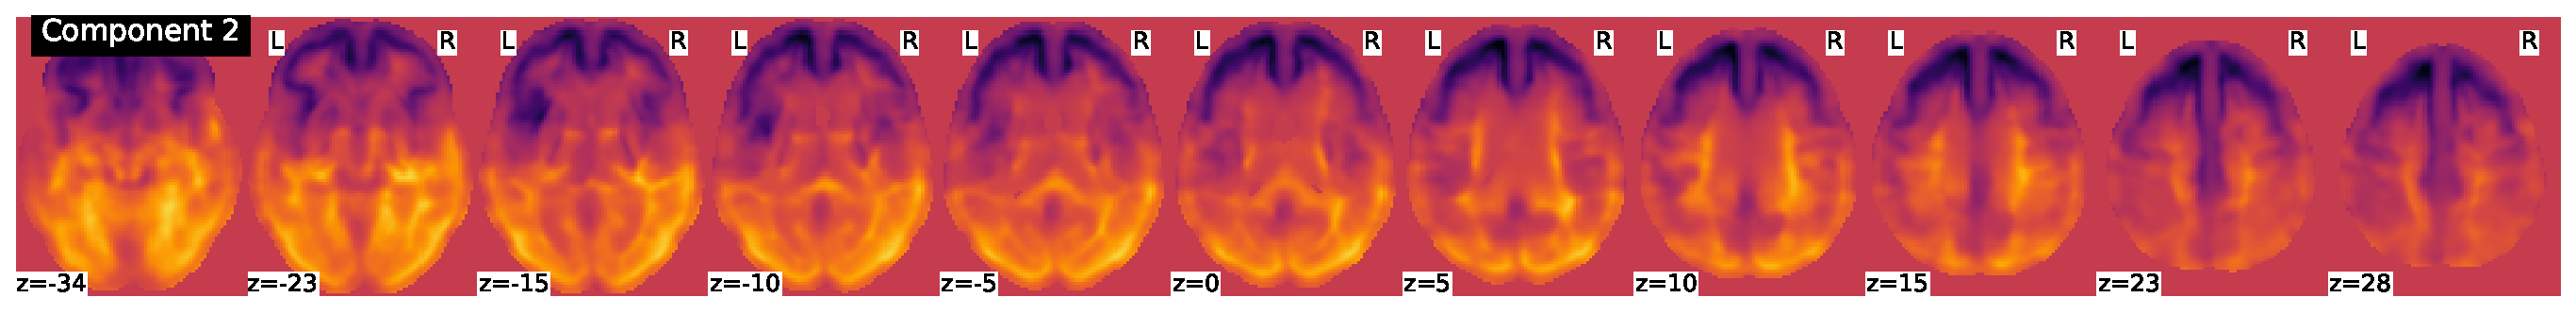
\includegraphics[width=0.9\linewidth]{Graphics/ch8/comp_2}
	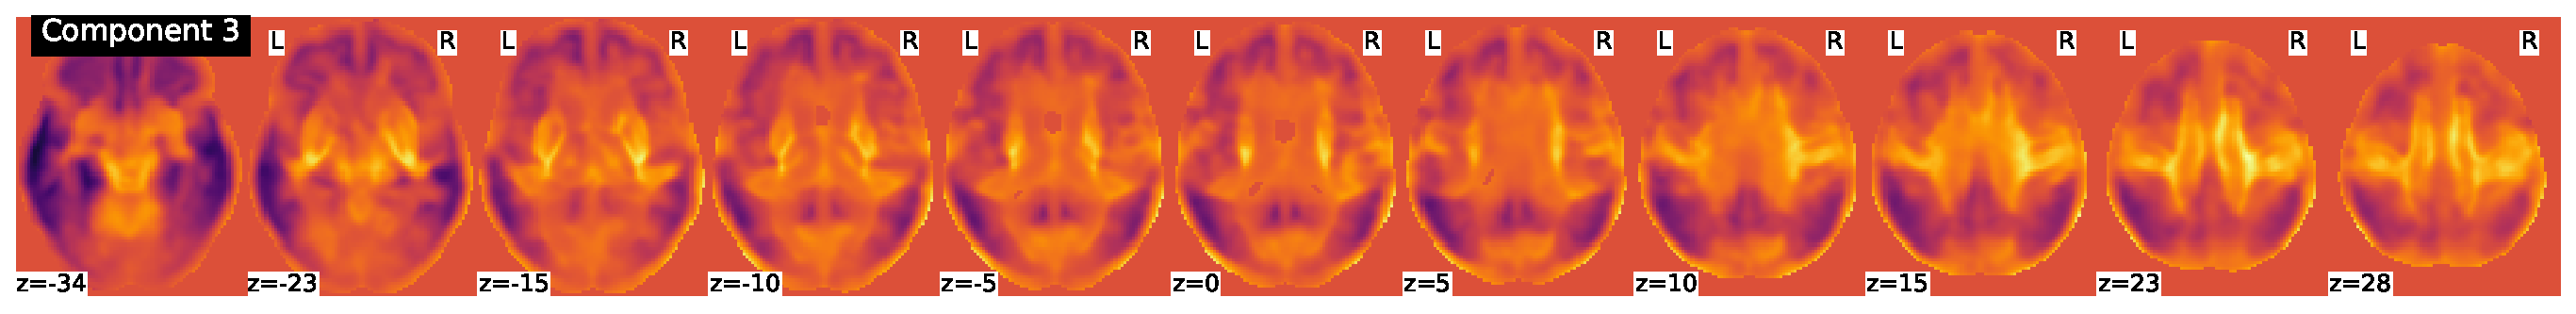
\includegraphics[width=0.9\linewidth]{Graphics/ch8/comp_3}
	\caption{Illustration of the three first eigenbrains in \acs{PCA}.}
	\label{fig:eigenbrainsSyn}
\end{figure*}

In Figure~\ref{fig:eigenbrainsSyn} we show the first four eigenbrains for the ADNI-PET dataset. We can see interesting patterns such as the contribution and size of ventricles in Component 0, the contrast in the cingulate gyri and precunei in Component 1, that have been widely documented \cite{Stoeckel04,Illan2011}. We can also recognise the contrast in glucose metabolism at the occipital lobe and some temporal and parietal negative influence encoded in Components 2 and 3. These features prove that the computed eigenbrains are representative of independent structures and activities that together can positively influence the synthesis of new brain images via a correct parametrization and estimation of the component scores. 


\begin{figure*}[h]
	\centering
	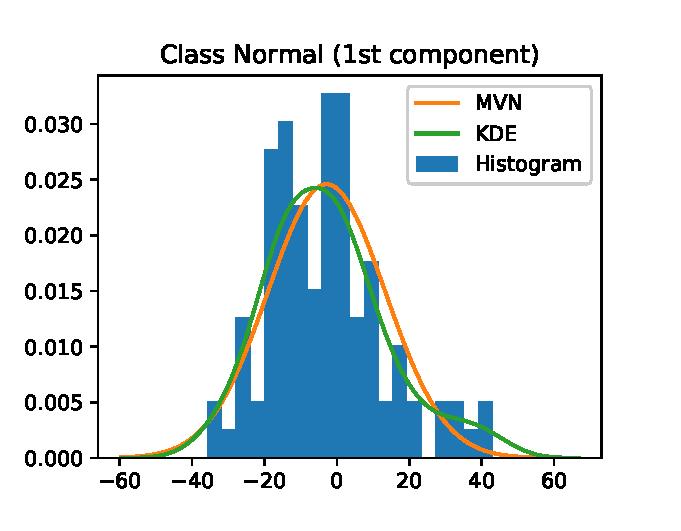
\includegraphics[width=0.3\linewidth]{Graphics/ch8/compMethods_Normal1st}
	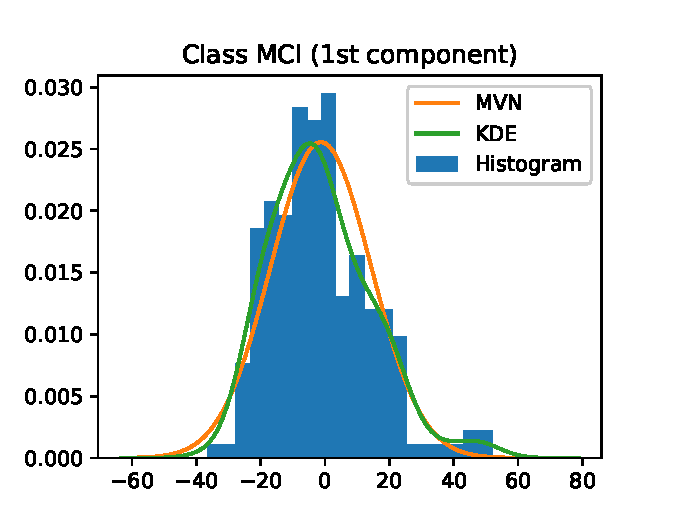
\includegraphics[width=0.3\linewidth]{Graphics/ch8/compMethods_MCI1st}
	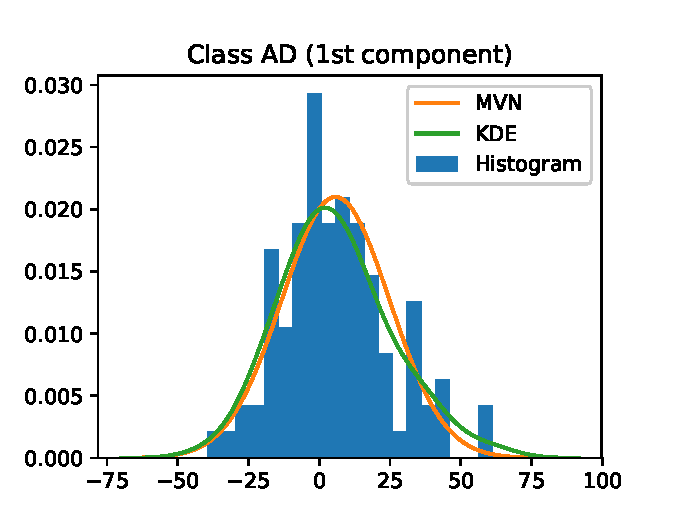
\includegraphics[width=0.3\linewidth]{Graphics/ch8/compMethods_AD1st}
	\caption{Comparison between the \acs{MVN} and \acs{KDE} \acs{PDF} estimation methods for the first component and the three groups, setting the histogram as reference.}
	\label{fig:comparisonEstimatesSyn}
\end{figure*}

% PDF estimation
Here is were we compare the two different estimation methods proposed: a \acf{MVN} and the \acf{KDE} via difussion. An accurate estimation of the distribution of the scores belonging to a certain class is paramount to obtain a reliable brain image synthesis. In Figure~\ref{fig:comparisonEstimatesSyn}, we compare the different estimation methods for the three \ac{AD} classes (in the first eigenbrain), using the histogram as a reference. We can see that, while the \ac{KDE} adapts more to the data, the \ac{MVN} is more general. This is for the first eigenbrain, but in Figure~\ref{fig:pairplot}, we can see the distribution of the first four scores in all groups, in which we can see that some of them (especially for eigenbrain 1 and 3), the distributions of some groups are less gaussian, and therefore, \ac{KDE} adapts better to this. Conversely, \ac{KDE} models each component independently, whereas the \ac{MVN} creates a parametric distribution of the scores of all eigenbrains, which could be considered an advantage. 

\begin{figure*}[h]
	\centering
	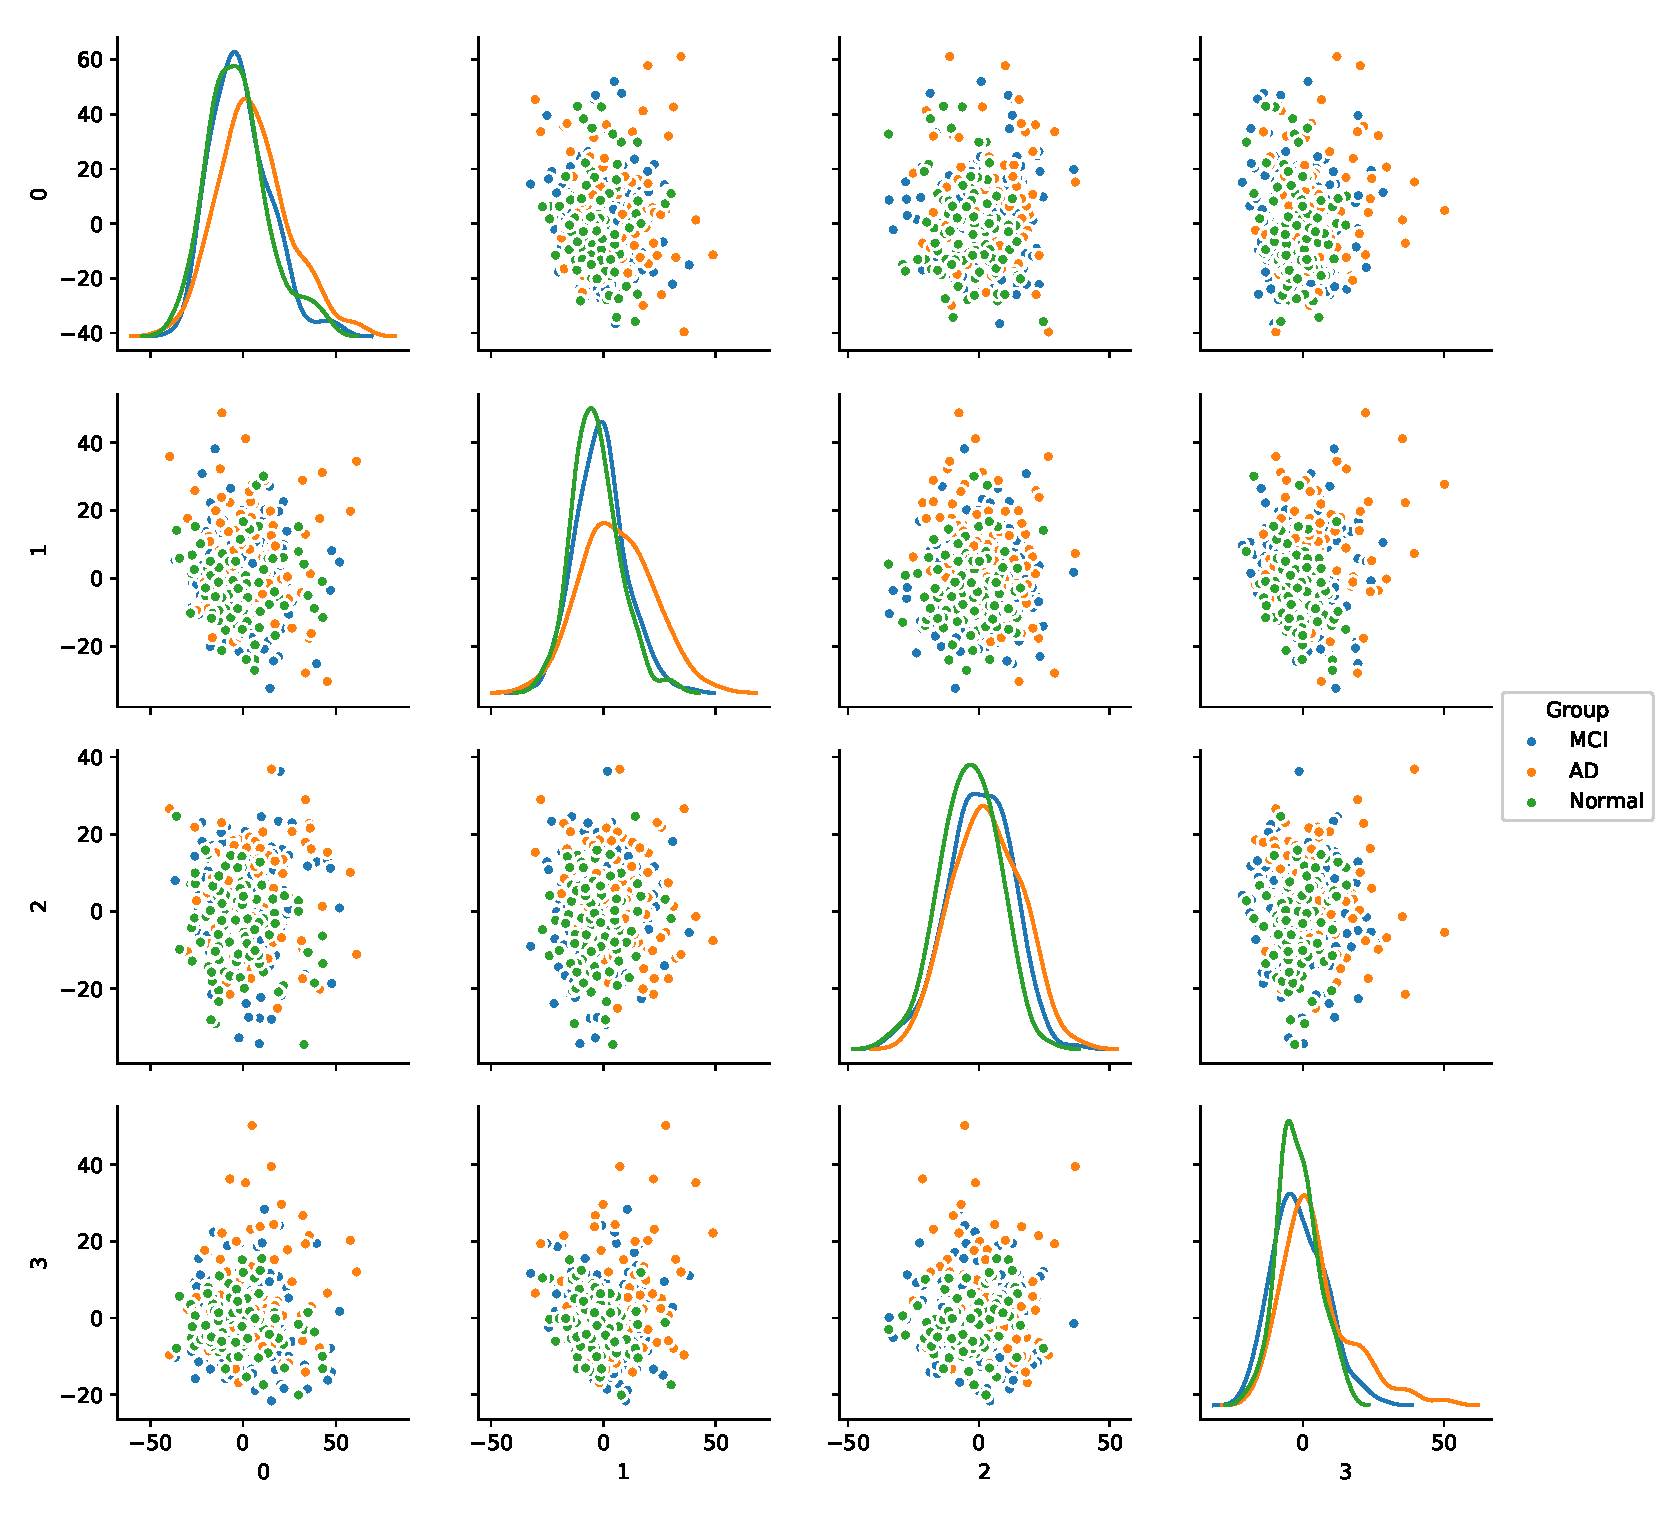
\includegraphics[width=\linewidth]{Graphics/ch8/Pairplot}
	\caption{Pairplot plotting the coordinates of the subjects in the ADNI-PET database over the four first eigenbrains. In the diagonal, distribution of the classes estimated using \acs{KDE} for each eigenbrain.}
	\label{fig:pairplot}
\end{figure*}

\begin{figure*}[h]
	\centering
	\includegraphics[width=0.9\linewidth]{Graphics/ch8/AD_nor_orig}
	\includegraphics[width=0.9\linewidth]{Graphics/ch8/AD_nor_sim_mvn}
	\includegraphics[width=0.9\linewidth]{Graphics/ch8/AD_nor_sim_kde}
	\includegraphics[width=0.9\linewidth]{Graphics/ch8/AD_ad_orig}
	\includegraphics[width=0.9\linewidth]{Graphics/ch8/AD_ad_sim_mvn}
	\includegraphics[width=0.9\linewidth]{Graphics/ch8/AD_ad_sim_kde}
	\caption{Examples of some original and simulated subjects from the ADNI-PET dataset.}
	\label{fig:samplesPET}
\end{figure*}

\begin{figure*}[h]
	\centering
	\includegraphics[width=0.9\linewidth]{Graphics/ch8/PKS_nor_orig}
	\includegraphics[width=0.9\linewidth]{Graphics/ch8/PKS_nor_sim_mvn}
	\includegraphics[width=0.9\linewidth]{Graphics/ch8/PKS_nor_sim_kde}
	\includegraphics[width=0.9\linewidth]{Graphics/ch8/PKS_pd_orig}
	\includegraphics[width=0.9\linewidth]{Graphics/ch8/PKS_pd_sim_mvn}
	\includegraphics[width=0.9\linewidth]{Graphics/ch8/PKS_pd_sim_kde}
	\caption{Examples of some original and simulated subjects from the PPMI dataset.}
	\label{fig:samplesDAT}
\end{figure*}

% Visual Analysis of the simulated images
A visual analysis of the synthesized images in Figures~\ref{fig:samplesPET} and \ref{fig:samplesDAT} reveals that the new images preserve similar characteristics of the original datasets. For example, it is easy to appreciate differences in glucose metabolism in Figure~\ref{fig:samplesPET} typically associated with \ac{AD}, such as a smaller activity at the temporal lobe or the striatum \cite{Stoeckel04,Illan2011}. In the simulated DaTSCAN images (Fig.~\ref{fig:samplesDAT}) differences in shape and intensity of the striatum, and bilateral differences \cite{Towey2011,Illan2012,martinez2014parametrization} can also be noticed, using both \ac{MVN} and \ac{KDE} modelling.

% Analysis of the SPM analysis 
To deepen the analysis of the synthesized figures, we will perform a \ac{SPM} analysis \cite{spm_book}, using the SPM12 software. In Figure~\ref{fig:spmAD}, we can look at the differences ($t$-maps, FWE corrected, $p<0.05$) between \ac{AD} and \ac{CTL} images with the original, and two synthesized datasets with 200 samples per class, using either \ac{MVN} or \ac{KDE} modelling. In these maps, the differences are located in similar places in both synthesized databases, that are as well, although less intense, represented in the \ac{SPM} analysis of the original dataset. The aforementioned regions such as the precuneus, angular, mid-temporal lobe, hippocampus, amygdala, among others, are represented in both the original and simulated datasets, in both the \ac{CTL} vs \ac{AD} (fig.~\ref{fig:spmAD}) and \ac{MCI} vs \ac{AD} (fig.~\ref{fig:spmMCIvsAD}) scenarios, with a special mention to the cingulum, which also is the main difference in the \ac{MCI} vs \ac{CTL} (fig.~\ref{fig:spmNORvsMCI}). 

\begin{figure}
	\centering
	Original ADNI-PET images\\
	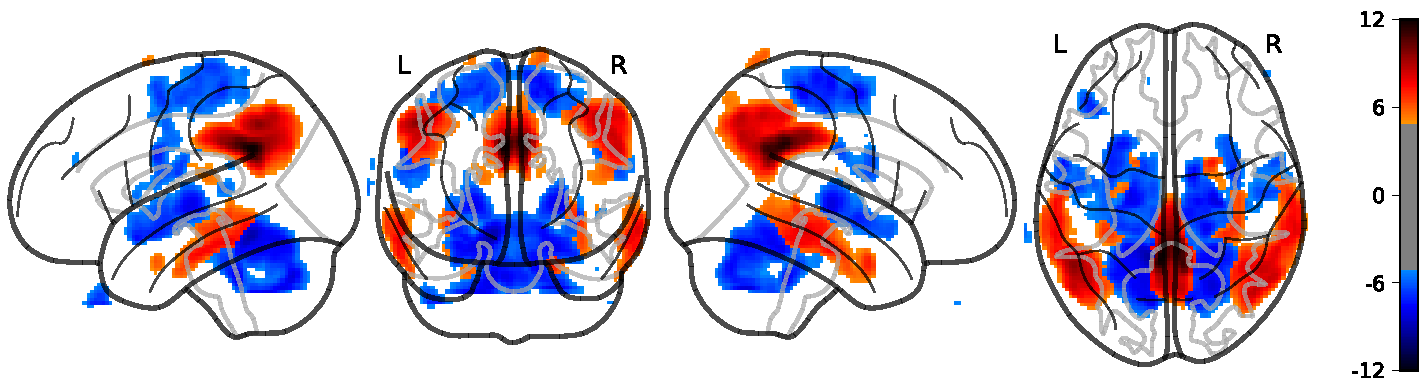
\includegraphics[width=\linewidth]{Graphics/ch8/NORvsAD_Orig_glass}\\
	\ac{MVN} Model\\
	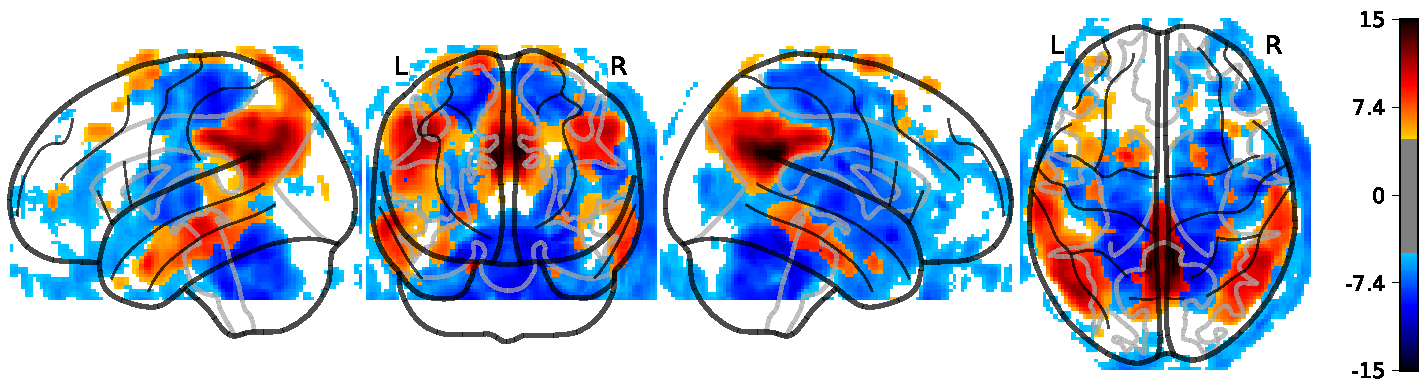
\includegraphics[width=\linewidth]{Graphics/ch8/NORvsAD_MVN_glass}\\
	\ac{KDE} Model\\
	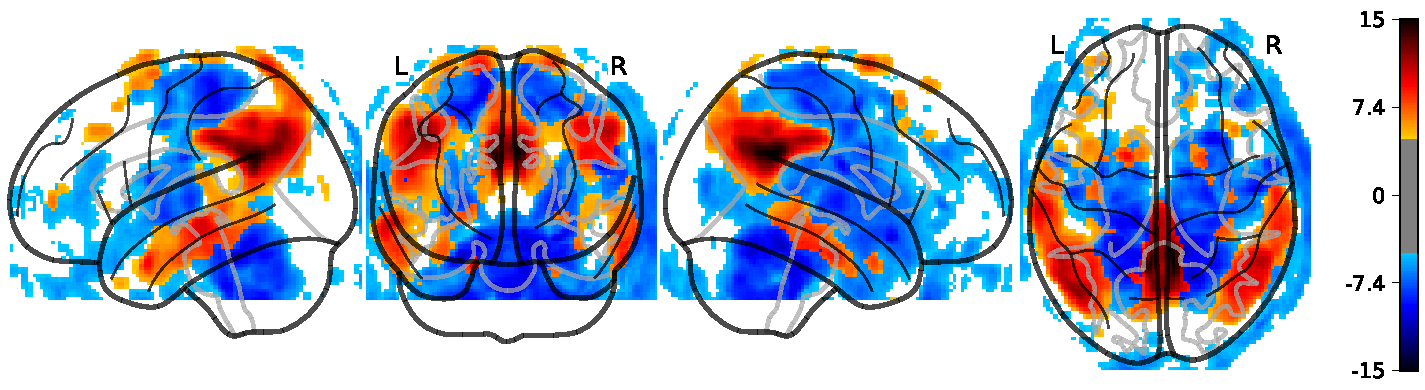
\includegraphics[width=\linewidth]{Graphics/ch8/NORvsAD_KDE_glass}
	\caption[\acs{SPM} Analysis of the ADNI dataset (\acs{AD} vs \acs{CTL}).]{\ac{SPM} Analysis of the ADNI dataset (\ac{AD} vs \ac{CTL}), \ac{FWE} corrected, with $p=0.05$, for the original and the simulated images.}
	\label{fig:spmAD}
\end{figure}


\begin{figure}
	\centering
	Original ADNI-PET images\\
	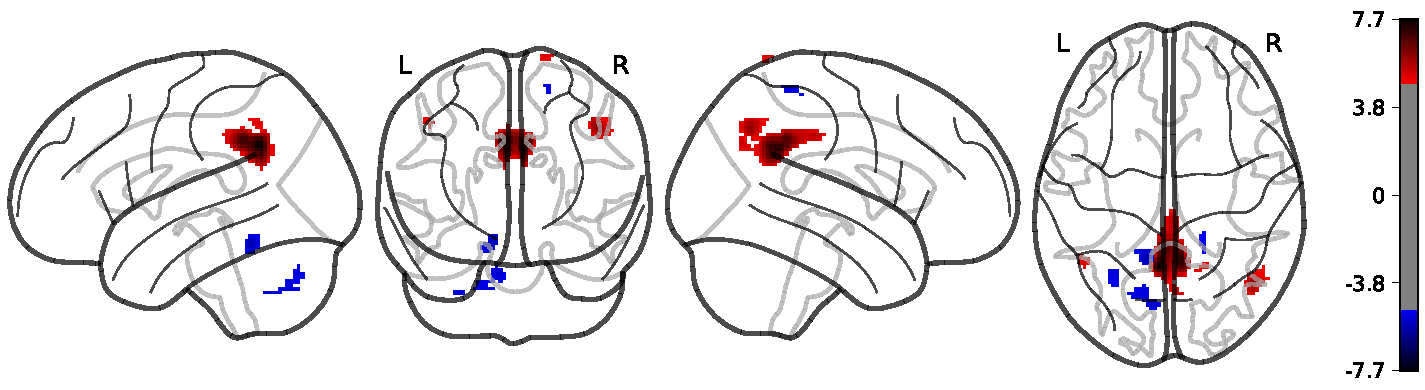
\includegraphics[width=\linewidth]{Graphics/ch8/NORvsMCI_Orig_glass}\\
	\ac{MVN} Model\\
	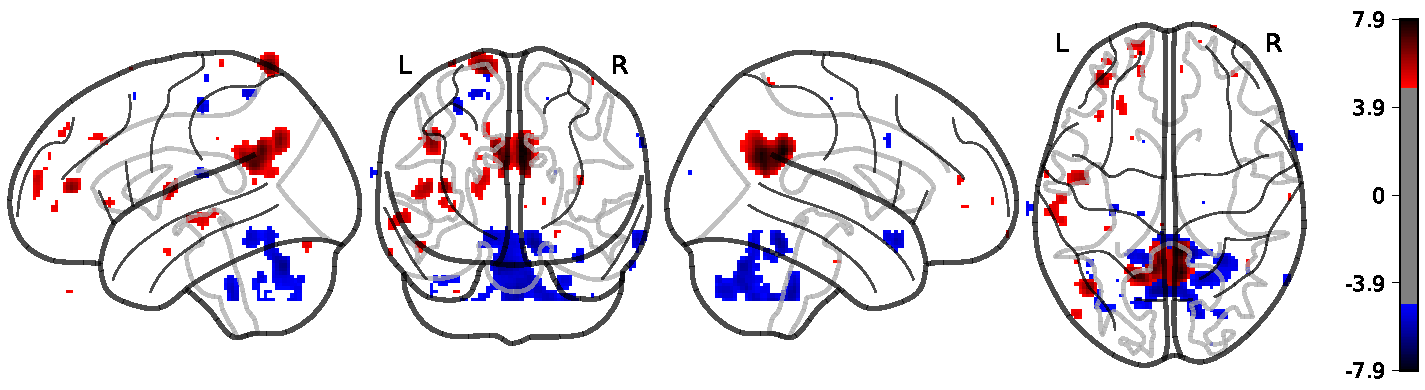
\includegraphics[width=\linewidth]{Graphics/ch8/NORvsMCI_MVN_glass}\\
	\ac{KDE} Model\\
	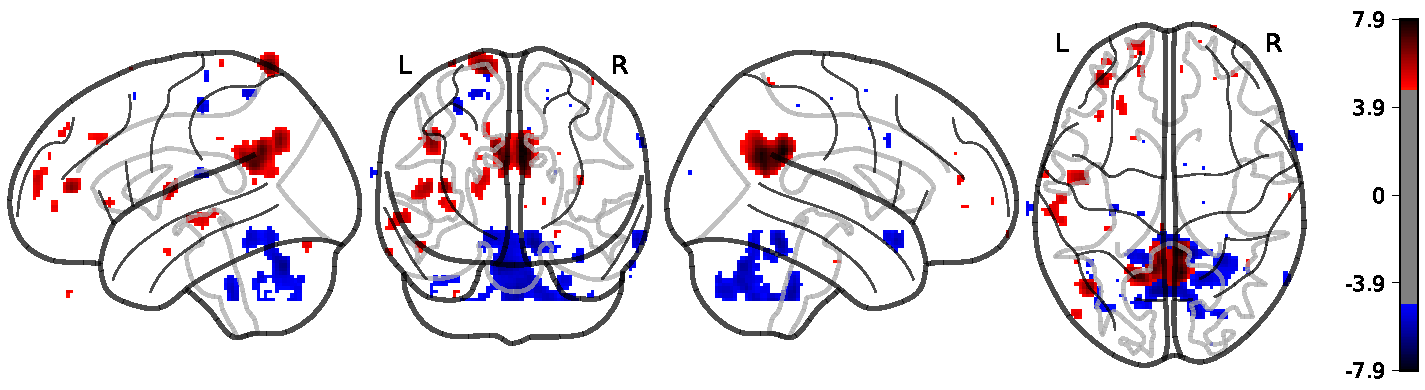
\includegraphics[width=\linewidth]{Graphics/ch8/NORvsMCI_KDE_glass}
	\caption[\acs{SPM} Analysis of the ADNI dataset (\acs{CTL} vs \acs{MCI}).]{\ac{SPM} Analysis of the ADNI dataset (\ac{CTL} vs \ac{MCI}), \ac{FWE} corrected, with $p=0.05$, for the original and the simulated images.}
	\label{fig:spmNORvsMCI}
\end{figure}


\begin{figure}
	\centering
	Original ADNI-PET images\\
	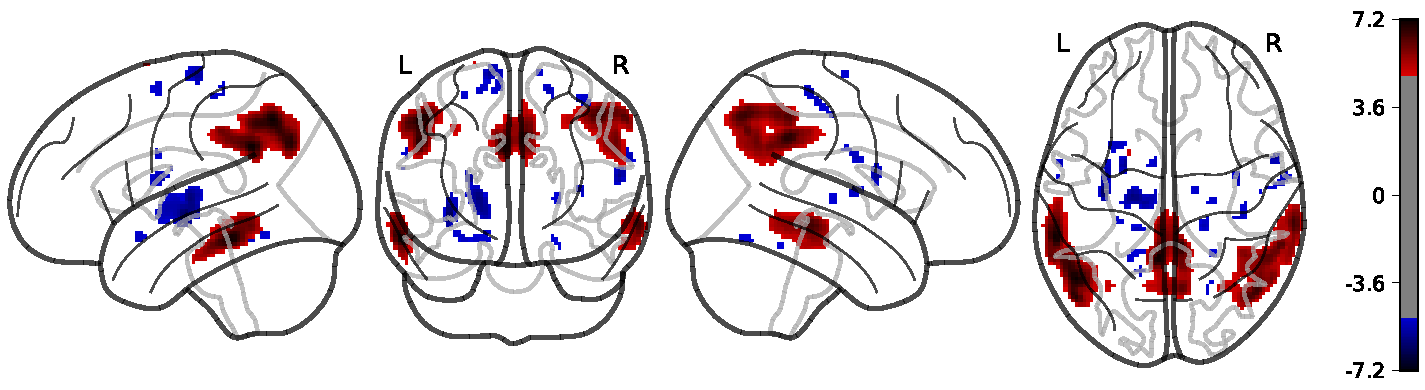
\includegraphics[width=\linewidth]{Graphics/ch8/MCIvsAD_Orig_glass}\\
	\ac{MVN} Model\\
	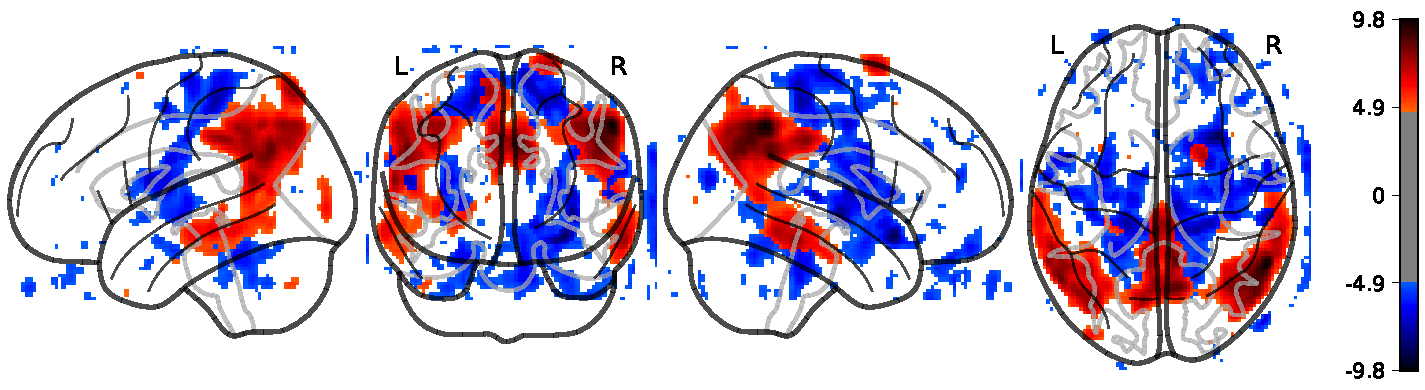
\includegraphics[width=\linewidth]{Graphics/ch8/MCIvsAD_MVN_glass}\\
	\ac{KDE} Model\\
	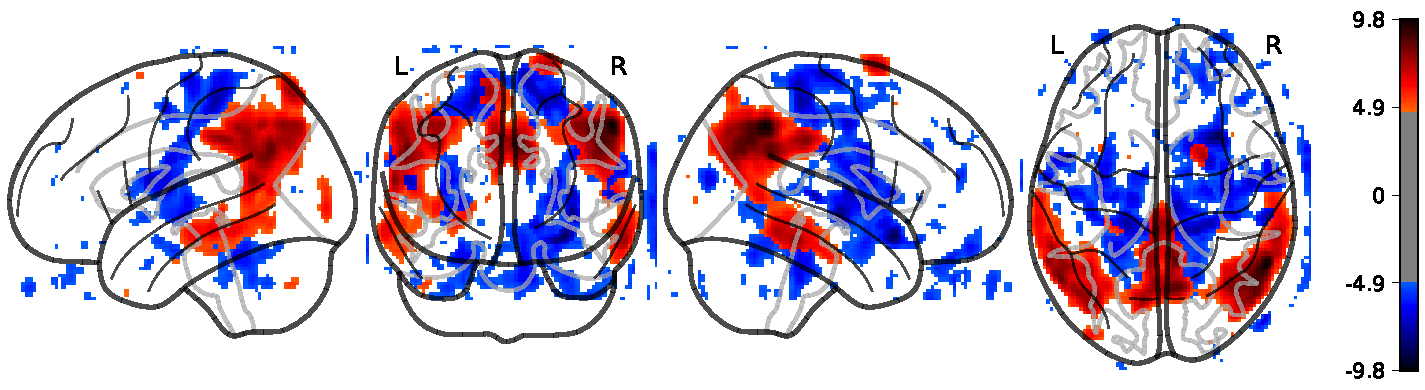
\includegraphics[width=\linewidth]{Graphics/ch8/MCIvsAD_KDE_glass}
	\caption[\acs{SPM} Analysis of the ADNI dataset (\acs{MCI} vs \acs{AD}).]{\ac{SPM} Analysis of the ADNI dataset (\ac{MCI} vs \ac{AD}), \ac{FWE} corrected, with $p=0.05$, for the original and the simulated images.}
	\label{fig:spmMCIvsAD}
\end{figure}

In the PPMI dataset, the \ac{SPM} analysis revealed (Figure~\ref{fig:spmPKS}) that the main differences are located in the posterior part of the striatum, specifically at the posterior part of the putamen and globus pallidus. This behaviour is consistent in both original and synthesized images, although with more statistical significance in the case of the \ac{MVN} model, and a more homogeneous distribution of the negative differences under the \ac{KDE} model. 


\begin{figure}
	\centering
	Original PPMI-DAT images\\
	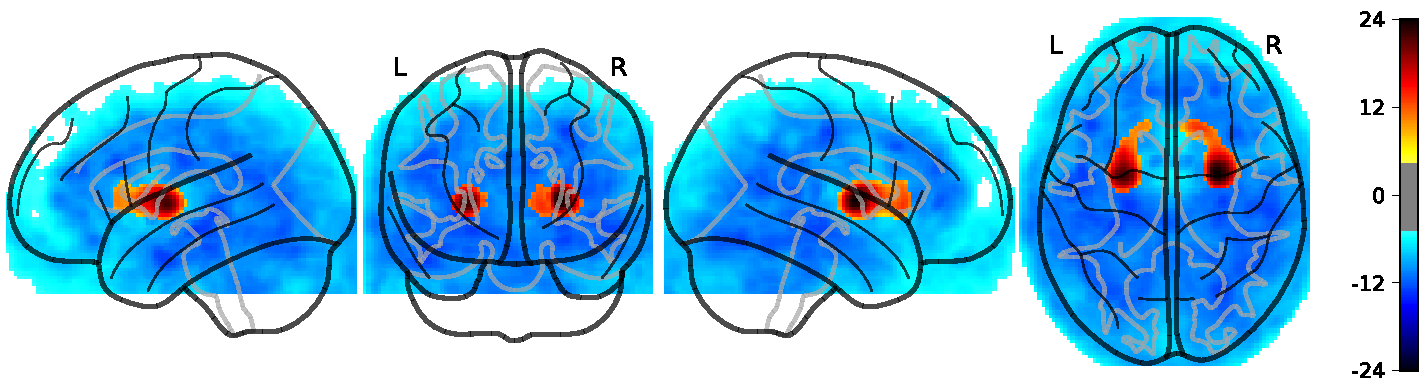
\includegraphics[width=\linewidth]{Graphics/ch8/NORvsPD_Orig_glass}\\
	\ac{MVN} Model\\
	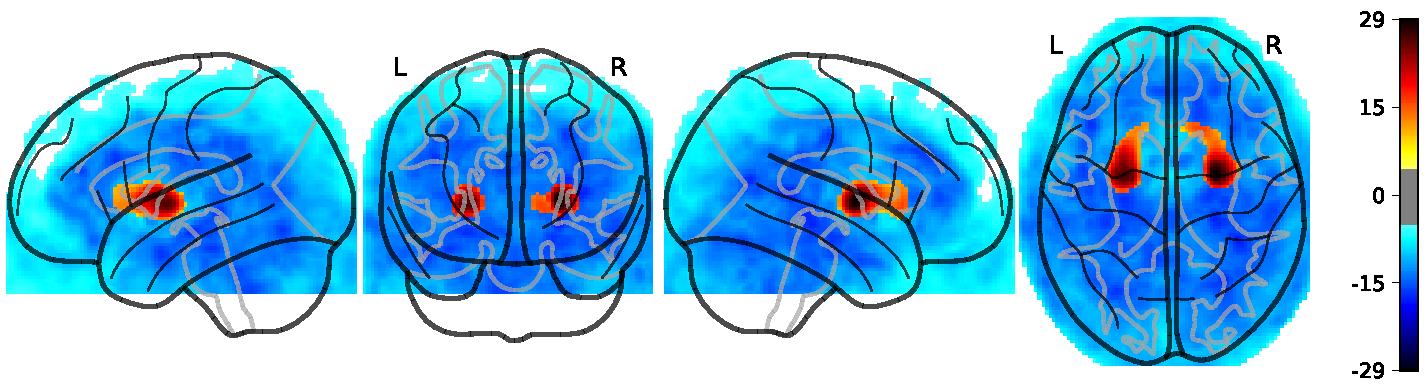
\includegraphics[width=\linewidth]{Graphics/ch8/NORvsPD_MVN_glass}\\
	\ac{KDE} Model\\
	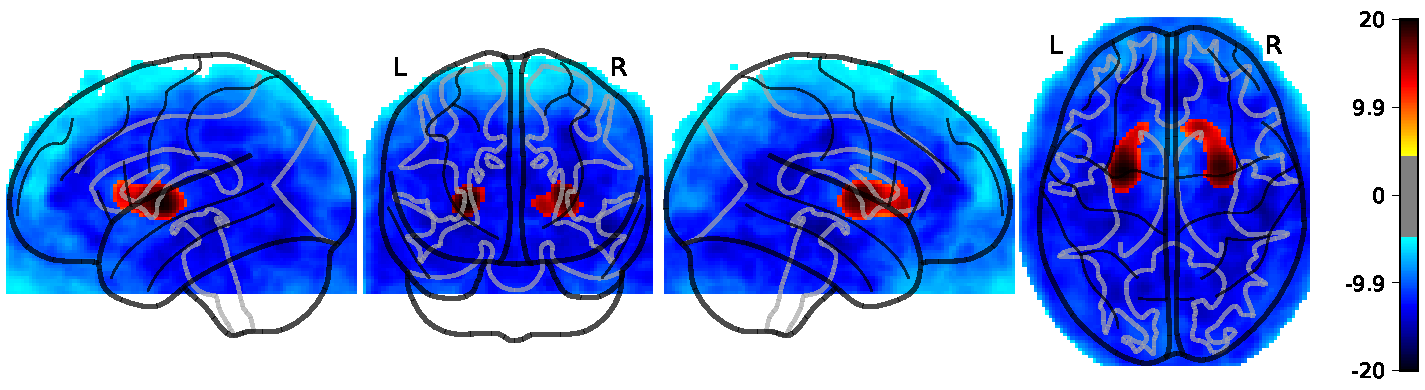
\includegraphics[width=\linewidth]{Graphics/ch8/NORvsPD_KDE_glass}
	\caption[\acs{SPM} Analysis of the PPMI dataset.]{\ac{SPM} Analysis of the PPMI dataset (\ac{PD} vs \ac{CTL}), \ac{FWE} corrected, with $p=0.05$, for the original and the simulated images.}
	\label{fig:spmPKS}
\end{figure}

% Analysis of the three experiments
As for the classification analysis, first we will compare the baseline performance of the simulated dataset with the original. From Table~\ref{tab:baselineSyn}, we can infer that \ac{MVN} produces minimally overlapping classes, whereas \ac{KDE} yields more similar images. This might be an indication of the more realistic distribution of classes when using \ac{KDE} modeling. Experiments 1 and 2 will give us more information on this.

First, in Experiment 1, we tested the predictive power of the simulated images. In this case, the SVC is trained with a set of simulated images, and then real images from the original dataset are predicted. In this case, we obtain higher accuracy when using \ac{MVN} modelling. This could point to either a more similar distribution of the synthesized images on the eigenbrain space, or a better definition of the support vectors of the decision plane of the classifier. In the first case, that would mean that the images synthesized using \ac{MVN} would be more similar to the original dataset. On the other hand, the decision plane could be better defined due to more concentrated classes, as hinted in the baseline experiment. For its part, the \ac{KDE} synthesis produces more disperse classes, which encompass the original dataset, degrading its performance in predicting the original dataset. 

Finally, Experiment 2 demonstrates the degree of similarity between the original and the synthesized images. To this purpose we train and test the classifier with the same subset of the original database. Then, we use that very subset to synthesize a new test set. The performance of this synthesized test set will give us an idea of how similar to the original dataset are our simulated images. From this experiment, we can see that the images simulated using \ac{MVN} achieved almost perfect accuracy when derived from the original training set, which could mean that there is almost no independence between the original and the simulated set. Conversely, the \ac{KDE} modelling produces significantly different images, in which the test performance decreases more than 15\% with respect to the original. This may indicate that these images are highly independent from the original dataset, although belonging to the same classes, as they achieved performances similar to the real-world baseline. 

% Best method. 
In conclusion, we can assume that the methodology producing the most real world images is the \ac{KDE} modelling. The images synthesized using this method are more similar to the real world images, in which we have more heterogeneous classes, and are in fact, less dependent on the dataset used as reference. However, all the results provided here prove that the simulated images can be safely used to increase sample size without losing predictive power, and the ones using \ac{KDE} can even introduce new behaviours that could compensate the false positives due to the small sample size problem. And these images could even be used in training environments for educational purposes, which is an inviting possibility. 